% Original book p4; original base PDF p8; input PDF p8; p004_s05 五、24点（五种结构）
% Role: question; original field: diagrams[0].tikz
% Compile with XeLaTeX from this figures/ directory.
\documentclass[12pt,tikz,border=5pt]{standalone}
\usepackage{fontspec}
\setmainfont[Path=../fonts/]{DroidSansFallback.ttf}
\setsansfont[Path=../fonts/]{DroidSansFallback.ttf}
\usepackage{amsmath,amssymb}
\usepackage{tikz}
\usetikzlibrary{calc,angles,quotes,arrows.meta,decorations.pathreplacing,decorations.pathmorphing,decorations.markings,patterns,positioning,fit,backgrounds,matrix,intersections,shapes.geometric}
\begin{document}
\color{black}
\tikzset{every picture/.append style={color=black}}
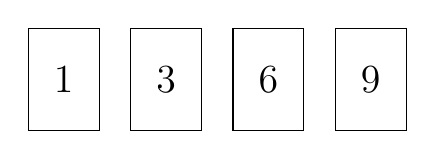
\begin{tikzpicture}\foreach \x/\v in {0/1,1.3/3,2.6/6,3.9/9}{\draw(\x,0)rectangle++(.9,1.3);\node at(\x+.45,.65){\Large\v};}\end{tikzpicture}

\end{document}
